\section{Model}\label{sec:Model}
%===========================================
This section presents a one-period trading model à la \citet{kyle1985continuous} with delegated asset management. 

\subsection{Setting}
The economy consists of a \textit{fund manager}, a competitive \textit{market maker}, a \textit{noise trader}, and $n\ge 2$ of \textit{investors}. All players are risk neutral. The manager leverages her skill (defined later) to identify a single risky asset with potential mispricing, raises capital from investors, and allocates it between the risky asset and a risk-free asset with a zero interest rate.\footnote{We abstract away from information acquisition by individual investors and assume that they invest through a manager due to the lack of informational advantages. This assumption would be supported by, for example, information- or skill-acquisition costs, where only the fund manager acquires the skill at lower costs due to economies of scale (e.g., \citealp{garleanu2018efficiently}).}

%\paragraph{\normalfont{\textit{Skill.}}}
\subsubsection{Skill}
The manager can uncover more information about the asset's payoff than
the market maker, and we interpret it as her \textit{skill}. At the beginning of the period, the manager draws private information $s$ from a normal distribution with mean zero and variance $\omega_{s}$. Leveraging this information, she identifies an asset with payoff $\delta = \bar{\delta} + s$, where $\bar{\delta}$ is a publicly known mean payoff. Since the market maker does not observe $s$, her prior expectation of the asset's payoff is $\mathrm{E}[\delta]=\bar{\delta}+\mathrm{E}[s]=\bar{\delta}$, which is biased by $s$ from the informed manager's perspective. As the market maker would set a price $p=\mathrm{E}[\delta]=\bar{\delta}$ in the absence of trades, $s$ can be viewed as the asset's ``potential mispricing.''\footnote{$s$ is not the \textit{actual} mispricing because the market maker will take into consideration the presence of the informed manager; thus, $p$ will deviate from $\bar{\delta}$ in equilibrium.} Indeed, as shown later, the manager profits by buying the asset if $s>0$ (underpriced) and selling it if $s<0$ (overpriced); the larger the $|s|$, the larger the profit. In light of this, we measure the manager’s \textit{realized} asset-selection skill by $|s|$, while the variance $\omega_s$ serves as an \textit{ex-ante} measure of the average skill.\footnote{This formalization of skill aligns with findings in the empirical studies that attribute fund managers' performance to stock-picking skills (e.g., \citealp{wermers2000mutual}; \citealp*{kosowski2006can}).}${}^{, }$\footnote{The definition of the average skill follows from $\mathrm{E}[|s|] = \omega_s \sqrt{\frac{2}{\pi_0}}$, where $\pi_0$ denotes the circular constant.}

\subsubsection{Capital Allocation and Trading}

\begin{figure}
\centering
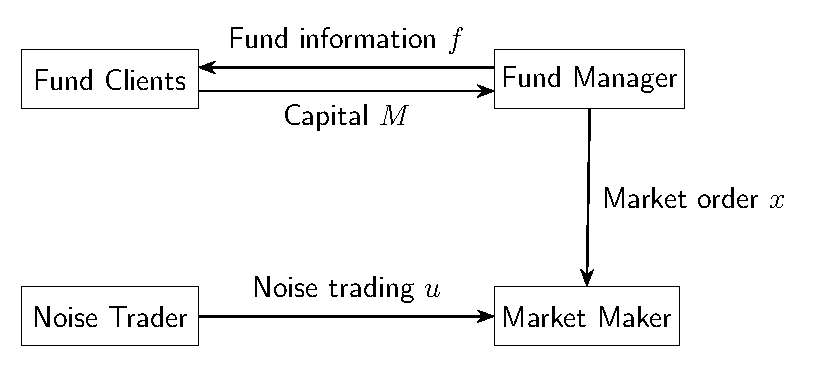
\includegraphics[width=0.65\linewidth]{./Figures/Fig_model.pdf}
\caption{Capital Allocation and Investment}\label{fig:model}
\end{figure}

We model the manager’s trading decision and investors' capital allocation as a simultaneous game with rational expectations, as illustrated in Figure \ref{fig:model}.

\paragraph{\normalfont{\it{Manager's tradign decision.}}}
Upon discovering the mispricing in the asset ($s$), the fund manager chooses the portfolio allocation between the risky and the safe asset. This action is represented by a market order for $x\in \mathbb{R}$ units of the risky asset, submitted to the market maker in the financial market. The manager decides on $x$ by incorporating the reactions of the financial market (i.e., the asset price) and the capital inflow from her investors, as described in the following.

\paragraph{\normalfont{\it{Investors' capital allocation.}}}
Each investor chooses the amount of capital to invest into the fund. Investor $i$'s capital allocation is denoted by $m_i \ge 0$, and the total fund flow or the asset under management (AUM) of the fund is defined by $M \equiv \sum_{i=1}^{n}m_{i}$. The fund’s fee structure is proportional to the total fund proceeds: the manager takes a $\phi\in(0,1)$ fraction of the proceeds, while the remaining $1-\phi$ fraction is distributed to the investors in proportion to their contributions to the fund, i.e., $m_i / M$.\footnote{Introducing a fixed fee does not change our qualitative results, as long as the performance-based fee also exists, $0 < \phi < 1$.}

\paragraph{\normalfont{\it{Financial market.}}}
In the financial market, the market maker sets the asset price, $p$, based on the incoming order flow, $x+u$, where $u$ represents a random market order from the noise trader and follows a normal distribution with mean zero and variance $\omega_u$. Due to competition, the market maker sets a semi-strong efficient price conditional on $x+u$:\footnote{Assume that, on the equilibrium path, one competitive market maker trades the asset. As in \citet{kyle1985continuous}, competitively many market makers exist off the equilibrium path, ensuring a break-even price in the equilibrium.} 
\begin{equation}
p=\mathrm{E}[\delta|x+u].\label{p}
\end{equation}


\subsubsection{Fund Opacity}
At the fund-raising stage, the manager disseminates a private noisy signal about her trading strategy to investors, defined as $f = x + e$, where $e$ represents a normally distributed noise term with mean zero and variance $\omega_{e}$.\footnote{We assume that $f$ is privately communicated between the manager and investors and is not observable to the market maker. Allowing the market maker to observe a noisy signal about $x$, however, does not affect the main qualitative results, as long as this signal differs from $f$, since the core results rely on the sensitivity of $p$ to $s$ being an increasing function of the manager's trading intensity.} This signal is referred to as the \textit{fund information}, and the noise variance of fund information, $\omega_e$, is used as the measure of \textit{fund opacity}. It describes the limited precision of the information that investors receive about the manager’s true trading strategy. A higher $\omega_{e}$ means that disclosed fund information is noisier, making the strategy harder to verify or reverse engineer. This reflects the idea that managers may deliberately obfuscate details by being vague, selective, or technically complex in their descriptions, while still engaging with investors to raise capital and to comply with disclosure rules.\footnote{For example, funds that largely track simple benchmark strategies are sometimes marketed using complex labels such as “dynamic opportunity,” “flexible growth,” or “adaptive allocation,” which convey sophistication while revealing little about actual portfolio construction. Similarly, managers may emphasize broad investment philosophies without clarifying how these translate into concrete portfolios.} Conversely, a lower $\omega_{e}$ corresponds to more transparent communication, allowing investors to form sharper beliefs about the manager’s actions.
Since the manager chooses her trading strategy $x$ based on the private signal $s$, the fund information $f$ is informative about the manager’s skill and the fund’s return. Thus, fund investors use $f$ to decide on their capital allocations. In what follows, we first consider the baseline model with exogenous opacity, while Section \ref{sec:endogenousopacity} endogenizes $\omega_{e}$ by allowing the manager to strategically choose fund opacity.

%\subsubsection{Misreporting and Verification.}
%\paragraph{\normalfont{\it{}}}
\subsubsection{Maximization Problems and Equilibrium}
The fund's profit from the risky investment is represented by $\pi\equiv(\delta-p)x$, so that the total fund proceeds, including those from the safe asset, are
\begin{equation}
    y=\pi+M.
\end{equation}
 %\paragraph{\normalfont{\it{Maximization problem.}}} 
Therefore, given the realized skill $s$, the fund manager maximizes her expected fee income by controlling her investment strategy $x$:
\begin{equation}
    \max_{x} \mathrm{E}\left[\phi y |s\right].\label{eq:managerproblem}
\end{equation}
Conversely, conditional on the fund information $f$, investor $i$ maximizes her expected return from delegating capital management:\footnote{The fund manager may have an incentive to make a false report about $y$ to her investors. Namely, by reporting $\tilde{y}$, she pays out $(1-\phi)\tilde{y}$ to investors and captures $y-(1-\phi)\tilde{y}$ on her own. To prevent this intentional misreporting, we assume that each investor can verify $x$ after the trading stage. Alternatively, we may assume costly verification: investors collectively pay the verification cost $C$ to back out $x$ from the fund information in the end of the trading period. As long as $C$ positively depends on the degree of fund opacity $\omega_e$, our qualitative results remain the same.}
\begin{equation}
    \max_{m_i\ge 0}\mathrm{E}\left[\frac{m_i}{M}(1-\phi)y -m_{i}|f\right].\label{eq:investorproblem}
\end{equation}
Note that the first term represents the expected payment from the fund, and the second term is the cost of capital.

\begin{definition}\label{def:eqm}
    The equilibrium is defined by the market maker's pricing strategy $p$, the fund manager's trading strategy $x$, and investors' capital allocations $\{m_{i}\}_{i=1}^{n}$, such that, (i) $p$ satisfies \eqref{p} given $x+u$, (ii) $x$ solves (\ref{eq:managerproblem}) given $s$, $p$, and $\{m_{i}\}_{i=1}^{n}$, and (iii) for all $i$, $m_i$ solves (\ref{eq:investorproblem}) given $p$, $f$, and $\{m_j\}_{j\neq i}$.

\end{definition} 
%*==*==*==*==*==*==*==*==*==*==*==*==*==*==*
\section{Equilibrium} \label{sec:eqm}
In this section, we search for a linear equilibrium in which the manager's market order $x$ is linear in her skill $s$, and the market maker's pricing strategy $p$ is also linear in the order flow $x+u$. Proofs for the analytical results are provided in the \hyperref[app:appendix]{Appendix}.

%===========================================
\subsection{Trading Strategy} \label{ss:conjecture}
Conjecture and later verify that the manager's equilibrium trading strategy is
\begin{equation}
 x(s)=\beta s,\label{x_conj}
\end{equation}
where $\beta>0$ is an endogenous constant determined in the equilibrium. Conjecture \eqref{x_conj} states that the manager buys (sells) the asset if her $s$ is positive (negative), where the order size is proportional to her skill $|s|$; the more skilled the manager, the more aggressively she trades.\footnote{This conjecture follows from the original Kyle model where an informed trader trades based on the difference between her belief and that of the market maker, i.e., $ \mathrm{E}[\delta|s]-\mathrm{E}[\delta] = s$.} The scale factor $\beta$ is referred to as the {\it trading intensity}, representing how intensively the manager exploits her informational advantage over the market maker.

%===========================================
\subsection{Execution Price} \label{ss:price}
The market maker decides on the price of the asset by extracting information about the asset's payoff from the aggregate order flow $x+u$. Anticipating the trading strategy \eqref{x_conj}, the price in equation \eqref{p} can be rewritten as
\begin{equation}
p=\bar{\delta}+\lambda(x+u),\label{eq:p}
\end{equation}
where
\begin{equation}
\lambda\equiv \frac{\beta \omega_{s}}{\beta^{2} \omega_{s}+\omega_{u}}\label{lambda}
\end{equation}
is referred to as ``Kyle's lambda,'' a measure of the price impact of order flow.\footnote{Since the market maker believes that the manager follows \eqref{x_conj}, the linear filtering rule with normally distributed random variables yields $p=\mathrm{E}[\bar{\delta} + s|\beta s + u] = \bar{\delta}+\mathrm{E}[s]+\frac{\mathrm{Cov}[s,\beta s+u]}{\mathrm{Var}[\beta s+u]}(x+u-\mathrm{E}[\beta s+u])=\bar{\delta}+\frac{\beta \omega_{s}}{\beta^{2} \omega_{s}+\omega_{u}}(x+u)$.} Following the literature, we define a market to be {\it liquid} if $\lambda$ is small.
%\footnote{From \eqref{p}, we have $p=\mathrm{E}[\delta|x+u]=\mathrm{E}[\mathrm{E}[\delta|x+u,s]|x+u]=\mathrm{E}[\bar{\delta}+s|x+u]$. Since the market maker believes that the manager follows \eqref{x_conj}, $s$ and $x+u$ are both normally distributed from the market maker's perspective. Thus, $p=\bar{\delta}+\mathrm{E}[s]+\frac{\mathrm{Cov}[s,x+u]}{\mathrm{Var}[x+u]}(x+u-\mathrm{E}[x+u])=\bar{\delta}+\frac{\mathrm{Cov}[s,\beta s+u]}{\mathrm{Var}[\beta s+u]}(x+u-\mathrm{E}[\beta s+u])=\bar{\delta}+\frac{\beta \omega_{s}}{\beta^{2} \omega_{s}+\omega_{u}}(x+u)$.}
%===========================================
\subsection{Investors' Capital Allocation} \label{ss:delegation}
By incorporating the fund proceeds $y = \pi + M$, investor $i$'s optimization problem in (\ref{eq:investorproblem}) is 
\begin{equation}
    \max_{m_i\ge 0} \frac{m_i}{M}(1-\phi)\mathrm{E}\left[\pi|f\right]-\phi m_i.\label{eq:mi_max}
\end{equation}
Investor $i$ solves this problem by incorporating the impact of her choice ($m_i$) on the total fund flow ($M$), while taking other investors' behavior ($\sum_{j\neq i} m_j$) as given. As she allocates a larger amount of capital, its marginal return diminishes due to the pro-rata allocation of the fund's proceeds, while the cost of capital linearly increases. This structure ensures the second-order condition of problem \eqref{eq:mi_max}, and the first-order condition pins down the optimal capital allocation as follows:
\begin{equation}
    m_{i}= \left(\frac{1-\phi}{\phi}\mathrm{E}[\pi|f]\sum_{j\neq i}m_j\right)^{\frac{1}{2}} -\sum_{j\neq i}m_j.
    \label{eq:mi}
\end{equation}
We focus on the symmetric equilibrium where all investors take the same action, $m_i = m$ for all $i=1,2,\cdots,n$. In this equilibrium, equation \eqref{eq:mi} reduces to 
\begin{equation}
    m = \frac{n-1}{n^2}\frac{1-\phi}{\phi}\mathrm{E}[\pi|f],\label{eq:m_sym}
\end{equation}
and the total fund flow becomes
\begin{equation}
    M \equiv n m = \theta \mathrm{E}[\pi|f],\label{eq:M_sym}
\end{equation}
where $\theta \equiv \frac{n-1}{n}\frac{1-\phi}{\phi}$ represents the \textit{flow-performance sensitivity}.  
Both the individual capital allocation and the total fund flow are linearly increasing in the expected trading profit conditional on the fund information, $\mathrm{E}[\pi|f]$. This is due to the performance-based fee structure, which makes the per-unit return from delegated asset management increasing in the trading profit. Also, equation (\ref{eq:M_sym}) specifies the flow-performance sensitivity $\theta$, which governs the reaction of the fund flow to the expected fund performance. The fund flow becomes less sensitive to the expected performance when the fee rate ($\phi$) is high, as high $\phi$ raises the cost of delegation and discourages investment, while it becomes more sensitive when the fund has a large clientele ($n$), as it attracts capital from a larger number of  investors.

\subsection{Reputation}
In determining the capital callocation in \eqref{eq:m_sym}, each investor seeks to compute the expected fund profits $\mathrm{E}[\pi|f]$. This process, in turn, requires the investor to back out the realized skill level of the manager $|s|$ from fund information $f=x+e$. 

% When the fund information is perfectly transparent (i.e., $\omega_{e}=0$), investors rationally use the trading strategy in \eqref{x_conj} and infer $s = x/\beta$, leading to\footnote{Given the linear pricing rule in \eqref{eq:p}, it holds that $\pi = (\delta - p)x = (s-\lambda \beta x)x$. Adopting trading strategy $x=\beta s$ leads to equation \eqref{eq:exp_pi_transparent}.}
% \begin{equation}
%       \mathrm{E}\left[\pi|f\right] = (1-\lambda \beta)\beta\mathrm{E}[s^2|s=x/\beta]=\left(\frac{1}{\beta}-\lambda\right)x^2.\label{eq:exp_pi_transparent}
% \end{equation}
% The first equality in (\ref{eq:exp_pi_transparent}) suggests that the fund return, $\pi=(\delta-p)x$, becomes a quadratic function of $s$, as both the manager's trading quantity $x$ and the profit margin, $\delta-p$, are proportional to the skill level in expectation. Furtheremore, the transparent fund information indicates that $s=x/\beta$, thereby shaping the conditional expected profit into quadratic in $x$, as the second equality in \eqref{eq:exp_pi_transparent} attests. 

% %This result implies that, on top of the maximizing profits, delegated asset management generates an additional incentive for the manager to control her trading strategy $x$, as it affects the total fund flow $M$ by influencing the investors' expectation about fund's returns.





% %===========================================
% \subsection{Manager's Optimization} \label{ss:optimization}
% By incorporating the total fund flow ([\ref{eq:M}] and [\ref{eq:exp_pi_transparent}]), the manager's problem in (\ref{eq:managerproblem}) is re-written as
% \begin{equation}
%     \max_{x} \phi\left(sx - \lambda x^2   + \theta\left(\frac{1}{\beta}-\lambda\right)x^2\right).\label{eq:managerproblem_transparent}
% \end{equation}
% The first two terms represent the fee income from the trading profit and are essentially identical to the trading profit in the original \citet{kyle1985continuous} model. The third term arises due to the fund inflow and, as equation (\ref{eq:exp_pi_transparent}) demonstrates, is determined by the quadratic size of risky investments. The optimal trading strategy solves \eqref{eq:managerproblem_transparent}, leading to
% \begin{equation}
%     x = \frac{1}{2}\frac{\beta}{\lambda\beta - \theta(1-\lambda\beta)}s.\label{eq:x=Fbeta}
% \end{equation}
% It is consistent with our guess in (\ref{x_conj}) when: 
% \begin{equation}
%     \beta = \frac{1}{2}\frac{\beta}{\lambda\beta - \theta(1-\lambda\beta)}.\label{eq:fixedpoint-transparent}
% \end{equation}
% By solving $\lambda$ and $\beta$ in equations (\ref{lambda}) and \eqref{eq:fixedpoint-transparent}, the trading strategy and the asset price are uniquely determined:
% \begin{lemma}\label{lem:transparent}
%     When the fund information is transparent ($\omega_{e}=0$), the manager's trading strategy and the asset price are specified by \eqref{x_conj} and \eqref{eq:p} with 
%     \begin{equation}
%         \beta = \sqrt{(1+2\theta)\frac{\omega_{u}}{\omega_{s}}},\label{eq:eqm_trade_transparent}
%     \end{equation}
%     and
%     \begin{equation}
%         \lambda = \frac{1}{2(1+\theta)}\sqrt{(1+2\theta)\frac{\omega_{s}}{\omega_{u}}}.\label{eq:eqm_lambda_transparent}
%     \end{equation}
% \end{lemma}
% %As is evident from problem (\ref{eq:managerproblem_transparent}), the flow-performance sensitivity, $\theta$, captures the manager's additional incentive to inflate her risky investment. 
% In the absence of delegated asset management ($\theta\rightarrow0$), the equilibrium is identical to the original \citet{kyle1985continuous} model, where $\beta$ is determined to maximize the expected trading profits. On one hand, the manager seeks to exploit her informational advantage by trading more intensively. On the other hand, it reveals information to the market maker and raises the price impact, cutting into the trading profit. The equilibrium $\beta$ balances these competing effects.

% Delegated asset management ($\theta>0$) brings about the additional risk-taking incentive, because inflating $x$ benefits the manager by making her appear highly skilled and inducing a larger fund flow (see equations [\ref{eq:M}] and [\ref{eq:exp_pi_transparent}]). We refer to this incentive as the ``showing-off'' motive. Since $\theta$ governs the flow-performance sensitivity, this motivation becomes stronger when $\theta$ is large, shaping equilibrium $\beta$ into an increasing function of $\theta$.

% Equation \eqref{eq:eqm_lambda_transparent} shows that the price impact $\lambda$ decreases with $\theta$. This is because the information is exaggerated in that the order size is too large relative to the true $|s|$ due to the showing-off motive. Thus, the market maker attempts to partially undo the manager's information revelation by incorporating less of it into the price, resulting in a weaker price impact.\footnotemark
% \footnotetext{\label{fn:footnote}$\lambda$ represents the price's reaction to the order flow $x+u$, rather than its reaction to the manager's private information $s$. The price impounds $s$ with coefficient $\beta\lambda$, which is monotonically increasing in $\theta$.}

% Our benchmark result in Lemma \ref{lem:transparent} isolates the fundamental mechanism through which delegated asset management enhances the manager’s risk taking behavior. The tendency of fund managers to show off their skill to attract capital is well discussed in the literature (e.g., \citealp{metrick2010economics}; \citealp*{chung2012pay}; \citealp{barber2017interim}), raising regulatory concerns that fund managers have incentives to exaggerate the performance or quality of their funds. In our model, however, a skilled manager may also have incentives to conceal her skill from the market maker, as emphasized by \citet{kyle1985continuous}. The next section explores how the fundamental tension between the showing off and the hiding motives shapes the equilibrium when the fund information becomes harder to interpret for investors due to opacity.